
\section{Application of Templates to Data}
\label{sec:data}

We select a signal region based on the expectation from MC that the fake MET in Z + jets becomes subdominant to the true MET in ttbar at a MET of approximately 60 GeV. In 11/pb, we find four events above this MET cut. [[?] A second signal region is chosen at a higher MET such that the expected yield is less than one event.]

The data and prediction overlayed with MC are shown in Fig.~\ref{fig:pfpred2} for Njet = 2, Fig.~\ref{fig:pfpredge2} for Njet $\ge$ 2, and Fig.~\ref{fig:pfpredge3} for Njet $\ge$ 3.

%note on my (Warren's) plot naming convention:
% the plots which have 'all' in the title are NOT binned in vsjp.
% ie 'pfMET_pred_2ge_alleb_log.png'
% I will leave the ones which are binned in vsjp in cvs, but remove from note (ie pfMET_pred_2_eb_log.png)

\begin{figure}[hbtp]
  \begin{center}
    \resizebox{1.0\linewidth}{!}{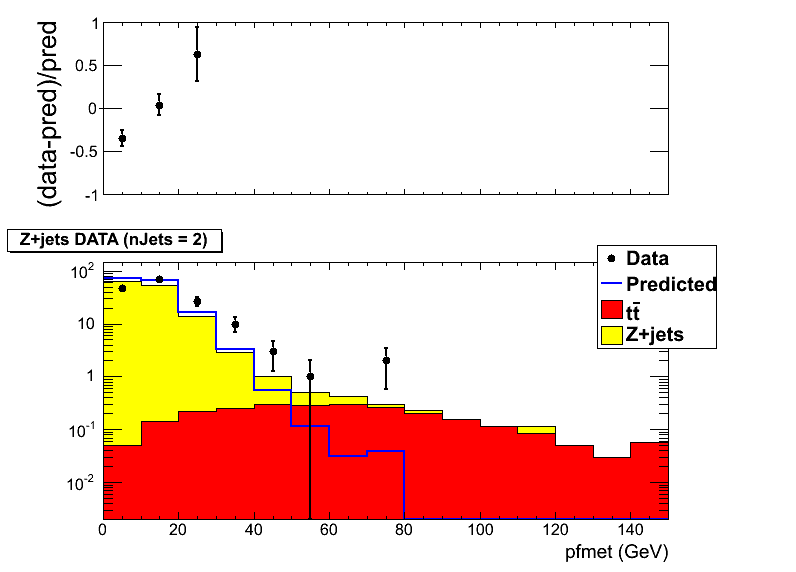
\includegraphics{plots/lep_metPredicted_njets1.png}}
	\\ \medskip 
    %\resizebox{\linewidth}{!}{
    \begin{tabular}{r|r|r}
      pfmet          & $>$ 30 & $>$ 60 \\ \hline
      data           &    16  &     2  \\
      pred           &  4.08  &  0.07  \\
      $Z$+jets MC    &  3.88  &  0.22  \\
      $t\bar{t}$ MC  &  2.10  &  1.27  \\
      $e\mu$         &     3     &  1  \\
   \end{tabular}
    \caption{The pfMET distribution for data (black points), prediction (solid blue line), and MC stacked for Njet $=$ 2. 
      The quantity (data-prediction)/prediction is shown on top of the plot.
      Below the plot is tabulated the integral of the data, prediction, and MC samples, as well as the yield in the $e\mu$
      final state, for pfMET $>$ 30~GeV and $>$ 60~GeV.
    }
    \label{fig:pfpred2}
  \end{center}
\end{figure}


%\begin{figure}[hbtp]
%  \begin{center}
%    \resizebox{0.75\linewidth}{!}{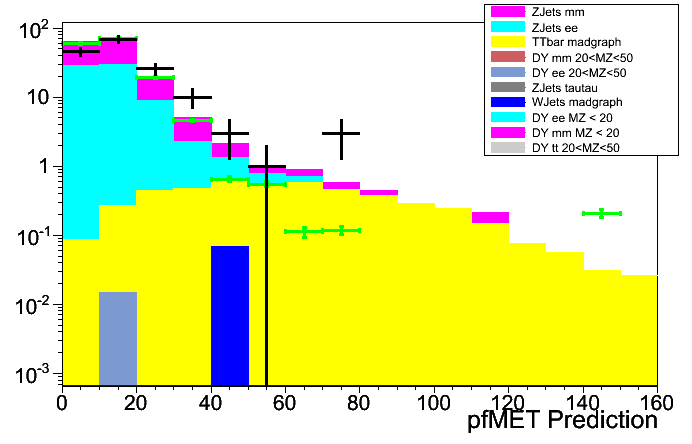
\includegraphics{plots/pfMET_pred_2_alleb_log.png}}
%	\\ \medskip 
%    %\resizebox{\linewidth}{!}{
%    \begin{tabular}{r|r|r}
%      pfmet & $>$ 30 & $>$ 60 \\ \hline
%   data&    17 &     3 \\
%  pred&  6.17 &  0.85 \\
%    MC& 11.10 &  2.92 \\
%   \end{tabular}
%	%}
%	\\ \medskip
%    \resizebox{0.5\linewidth}{!}{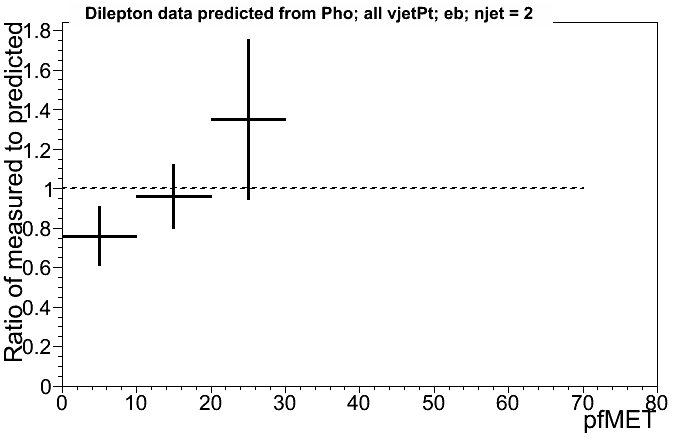
\includegraphics{plots/pfMET_pred_2_alleb_ratio.png}}
%    \caption{The pfMET distribution for data (black), prediction (green), and MC stacked for Njet $=$ 2. Below the plot is tabulated the integral of the data, prediction, and MC for pfMET $>$ 30 and $>$ 60. Finally, the ratio of predicted to measured pfMET is shown at the bottom.}
%    \label{fig:pfpred2}
%  \end{center}
%\end{figure}

\begin{figure}[hbtp]
  \begin{center}
    \resizebox{1.0\linewidth}{!}{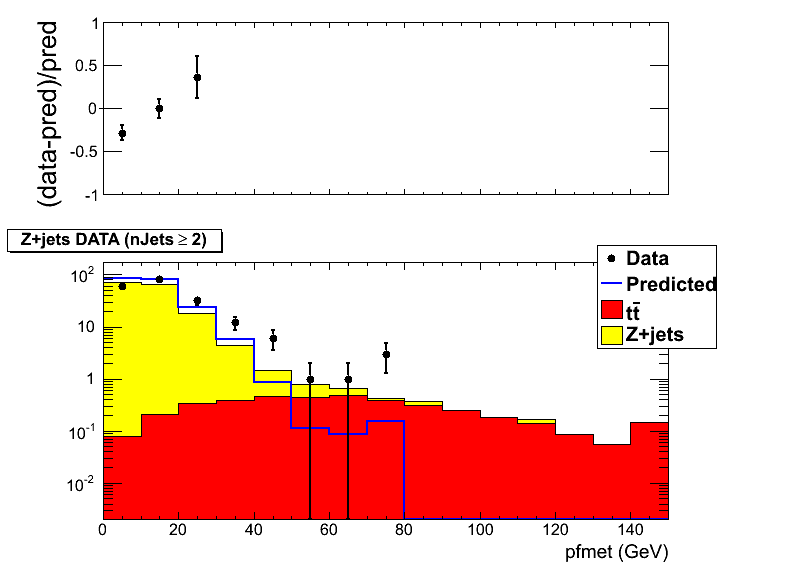
\includegraphics{plots/lep_metPredicted.png}}
	\\ \medskip 
    %\resizebox{\linewidth}{!}{
    \begin{tabular}{r|r|r}
      pfmet          & $>$ 30 & $>$ 60 \\ \hline
      data           &     23 &      4 \\
      pred           &   6.93 &   0.24 \\
      $Z$+jets MC    &   5.72 &   0.31 \\
      $t\bar{t}$ MC  &   3.35 &   2.05 \\
      $e\mu$         &      4 &      2  \\
   \end{tabular}
    \caption{The pfMET distribution for data (black points), prediction (solid blue line), and MC stacked for Njet $\ge$ 2. 
      The quantity (data-prediction)/prediction is shown on top of the plot.
      Below the plot is tabulated the integral of the data, prediction, and MC samples, as well as the yield in the $e\mu$
      final state, for pfMET $>$ 30~GeV and $>$ 60~GeV.
    }
    \label{fig:pfpredge2}
  \end{center}
\end{figure}

%\begin{figure}[hbtp]
%  \begin{center}
%    \resizebox{0.75\linewidth}{!}{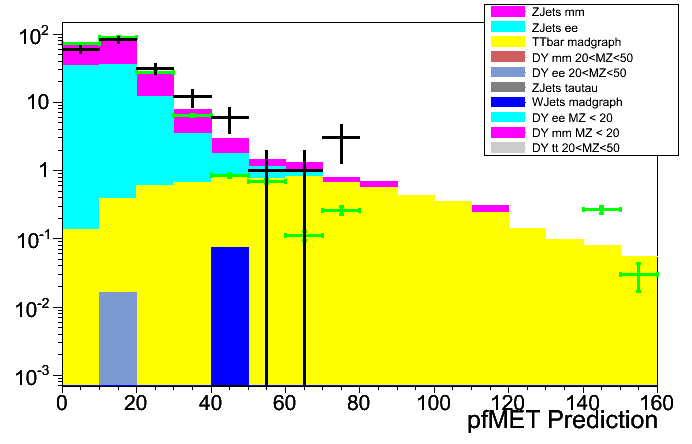
\includegraphics{plots/pfMET_pred_2ge_alleb_log.png}}
%	\\ \medskip 
%    %\resizebox{\linewidth}{!}{
%    \begin{tabular}{r|r|r}
%      pfmet & $>$ 30 & $>$ 60 \\ \hline
%  data&    23 &     4 \\
%  pred&  9.05 &  1.07 \\
%    MC& 16.66 &  4.40 \\
%    \end{tabular}
%	%}
%	\\ \medskip
%    \resizebox{0.5\linewidth}{!}{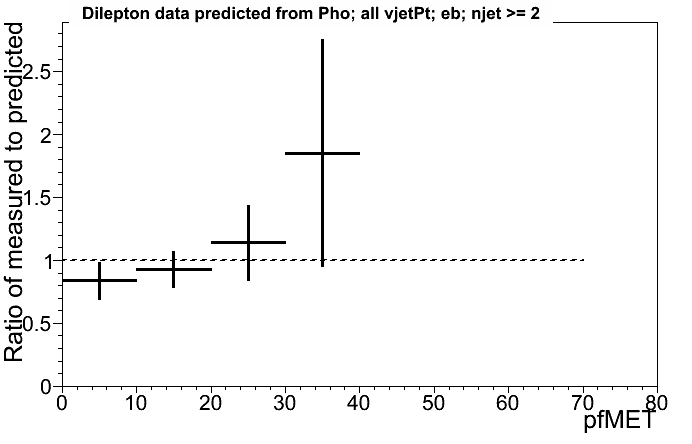
\includegraphics{plots/pfMET_pred_2ge_alleb_ratio.png}}
%    \caption{The pfMET distribution for data (black), prediction (green), and MC stacked for Njet $\ge$ 2. Below the plot is tabulated the integral of the data, prediction, and MC for pfMET $>$ 30 and $>$ 60. Finally, the ratio of predicted to measured pfMET is shown at the bottom.}
%    \label{fig:pfpredge2}
%  \end{center}
%\end{figure}

\begin{figure}[hbtp]
  \begin{center}
    \resizebox{1.0\linewidth}{!}{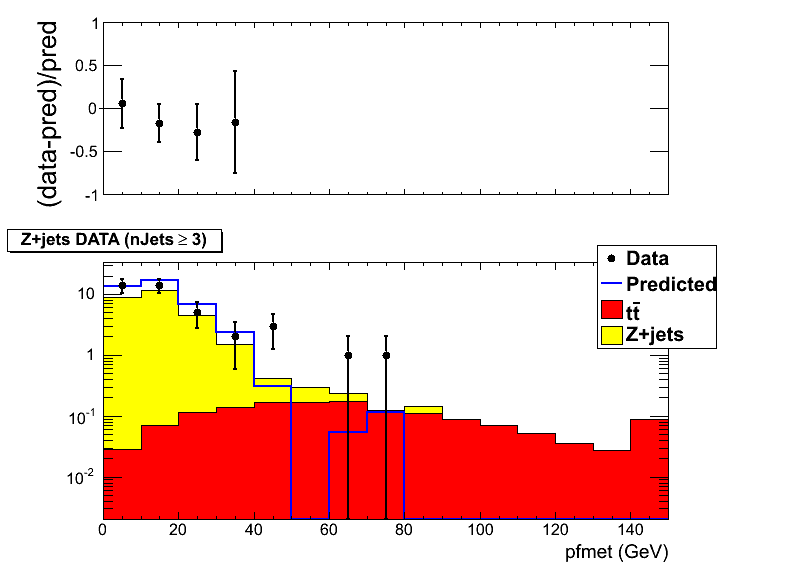
\includegraphics{plots/lep_metPredicted_njets2.png}}
	\\ \medskip 
    %\resizebox{\linewidth}{!}{
    \begin{tabular}{r|r|r}
      pfmet          & $>$ 30 & $>$ 60 \\ \hline
      data           &     7  &     2  \\
      pred           &  2.85  &  0.17  \\
      $Z$+jets MC    &  1.83  &  0.09  \\
      $t\bar{t}$ MC  &  1.25  &  0.77  \\
      $e\mu$         &     1  &     1  \\
   \end{tabular}
    \caption{The pfMET distribution for data (black points), prediction (solid blue line), and MC stacked for Njet $\ge$ 3. 
      The quantity (data-prediction)/prediction is shown on top of the plot.
      Below the plot is tabulated the integral of the data, prediction, and MC samples, as well as the yield in the $e\mu$
      final state, for pfMET $>$ 30~GeV and $>$ 60~GeV.
    }
    \label{fig:pfpredge3}
  \end{center}
\end{figure}

%\begin{figure}[hbtp]
%  \begin{center}
%    \resizebox{0.75\linewidth}{!}{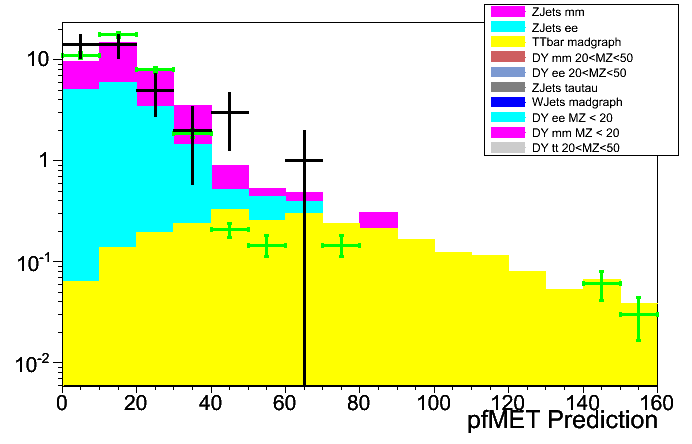
\includegraphics{plots/pfMET_pred_3ge_alleb_log.png}}
%	\\ \medskip
%    %\resizebox{\linewidth}{!}{
%    \begin{tabular}{r|r|r}
%      pfmet & $>$ 30 & $>$ 60 \\ \hline
%  data&     6 &     1 \\
%  pred&  2.88 &  0.21 \\
%    MC&  6.70 &  1.78 \\
%    \end{tabular}
%	%}
%	\\ \medskip
%    \resizebox{0.5\linewidth}{!}{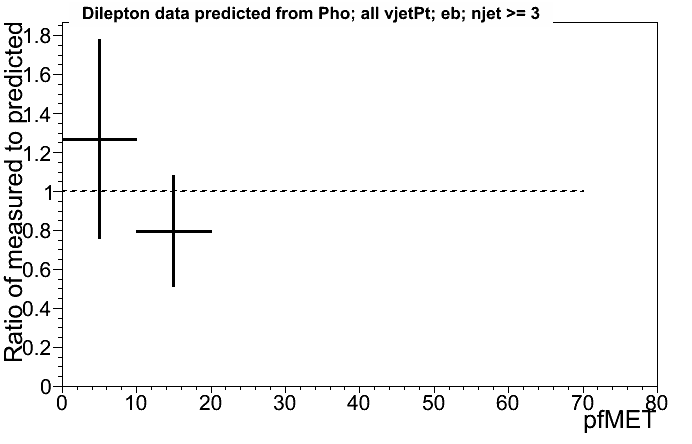
\includegraphics{plots/pfMET_pred_3ge_alleb_ratio.png}}
%    \caption{The pfMET distribution for data (black), prediction (green), and MC stacked for Njet $\ge$ 3. Below the plot is tabulated the integral of the data, prediction, and MC for pfMET $>$ 30 and $>$ 60. Finally, the ratio of predicted to measured pfMET is shown at the bottom.}
%    \label{fig:pfpredge3}
%  \end{center}
%\end{figure}


